\documentclass[a4paper,10pt]{article}
\usepackage[T2A]{fontenc}
\usepackage[utf8x]{inputenc}
\usepackage{ucs}
\usepackage{cmap}
\usepackage[english,russian]{babel}
\usepackage{amsmath}
\usepackage{color,graphicx}
\usepackage{indentfirst}
\usepackage{ucs} 
\usepackage[utf8x]{inputenc}

\title{SRM методичка}
\author{Чернышев Алексей}
\setlength{\parindent}{1cm}

\begin{document}
\section*{Спайковые НС}
\section*{Spike Responce Model}
\paragraph*{Общее описание. }Spike Responce Model (SRM) - наиболее популярная модель спайкового нейрона. SRM своей популярностью обязана простотой математической интерпретации - вся динамика нейрона описывается одним уравнением вида $u(t)$, которое описывает напряжение на мембране нейрона и, по сути, является решением дифференциального уравнения для моделей типа \textit{Integrate and fire}. Динамику моделей \textit{Integrate and fire} можно описать так: нейрон суммирует входные сигналы и по достижению определенного порога, производит спайк, после чего нейрон переходит в состояние рефракторности, находясь в котором, вероятность нового спайка крайне мала.\\
\indent Поведение описанное выше можно поэтапно собрать в одну формулу: 
\begin{enumerate}
\item \textit{Функция описывающая напряжение на синапсах}. В качестве такой функции можно взять альфа функцию с экспоненциальным подъёмом и спадом, причем подъем и спад наиболее натуральным будет взять быстрым и медленным соответственно. Типичный график подобной функции можно посмотреть на рисунке ниже:
\begin{figure}[ht]
\centering
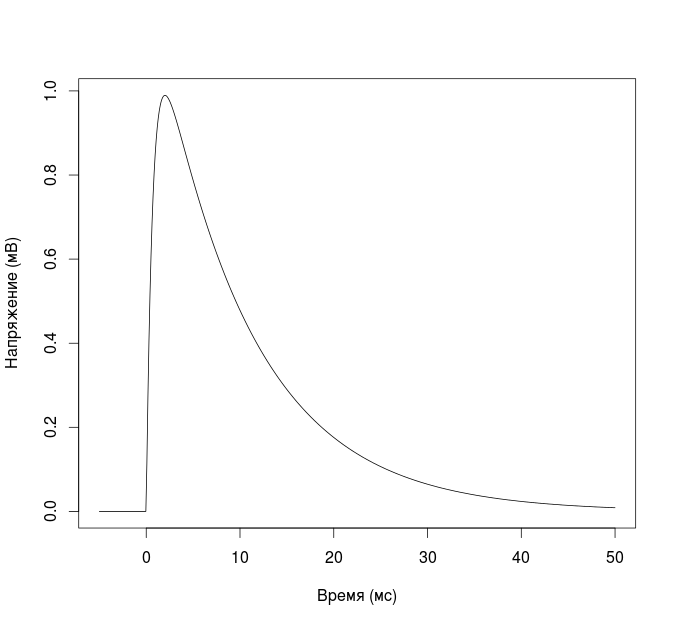
\includegraphics[width=0.75\linewidth]{epsp}
\caption{Потенциал на синапсах}
\end{figure} \\
Такая функция задается формулой:
\begin{equation}\label{eq:epsp}
\epsilon(t) =	\epsilon{0}(\exp(-t/t_{m})-\exp(-t/t_{s})),
\end{equation}
где $\epsilon{0} = 1.3$мВ - контанста задающая масштаб потенциала, $t_{m}=0.7$мс - константа отвечающая подъем, $t_{s} = 10$мс - константа отвечающая спад.

\item \textit{Функция описывающая рефракторность нейрона}. Основное требования к такой функции в том, чтобы напряжение на нейроне резко падало вниз, и потом медленно восстанавливалось. График подобной функции можно увидеть на рисунке ниже:
\begin{figure}[ht]
\centering
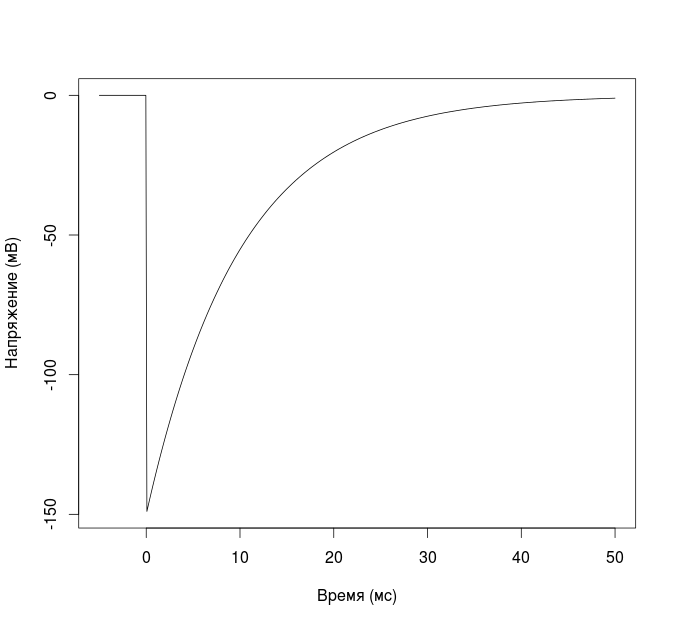
\includegraphics[width=0.75\linewidth]{nu}
\caption{Рефракторность нейрона}
\end{figure} \\
Здесь используется данная функция:
\begin{equation}\label{eq:nu}
\eta(t) =	\eta_{0}(-\exp(-t/t_{m})),
\end{equation}
где $\eta_{0} = -150$мВ - констанста описывающая минимальное напряжение на мембране, от которого идёт медленное восстановление, $t_{m}$ - скорость восстановления можно взять из функции синаптического потенциала, для простоты. 
\end{enumerate}
В итоге, используя эти функции, можно записать уравнение, которое будет описывать напряжение на мембране нейрона, причём: \\
\begin{itemize}
 \item Пусть нейрон $i$ имеет $N$ синапсов и у каждого синапса есть вес $w_{i}$, тогда напряжение на мембране в данный момент времени $t$ будет взвешенной суммой синаптических потенциалов: $\sum_{j=1}^N w_{j} \sum_{f_{j}} \epsilon_{j}(t-f_{j})$, где $f_{j}$ - время спайка на синапсе $j$. \\
\item Рефракторность нейрона будет простой суммой по всем спайкам, которые произвел нейрон $i$: $\sum_{f_{i}}\eta(t-f_{i})$
\item Нейрон имеет т.н. потенциал покоя. Биологические нейроны имеют разнообразные значения такого потенциала, как правило берут $u_{rest} = 70$ мВ.
\end{itemize}

\indent Таким образом получаем формулу, которая объединяет все вышеописанные особенности:
\begin{equation}\label{eq:u_srm}
u(t) = u_{rest} + \sum_{j=1}^N w_{j} \sum_{f_{j}} \epsilon_{j}(t-f_{j}) + \sum_{f_{i}}\eta(t-f_{i}),
\end{equation}
Типичный график иллюстрирующий работу функции \ref{eq:u_srm} ниже: 
\begin{figure}[ht]\label{pic:u_srm}
\centering
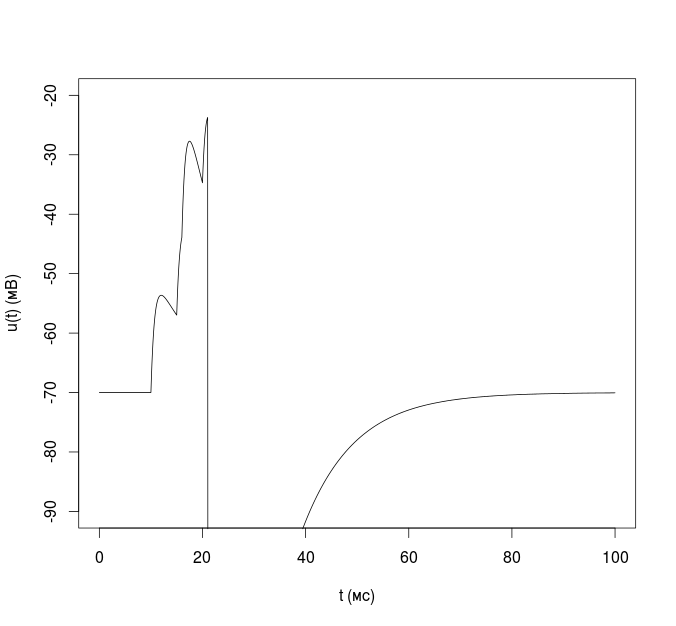
\includegraphics[width=1\linewidth]{u_srm}
\caption{Потенциал нейрона}
\end{figure} \\
\indent На рисунке представлен случай когда произошли спайки на двух синапсах во времена $f_{1} = \{10, 16\}$ и $f_{2}=\{15,20\}$, которые заставили нейрон произвести спайк в $f_{i} = \{21\}$. Веса были выбраны большими, для наглядности графика.
\paragraph*{Генерация спайков.} Модель описанная выше включает в себя только поведение при данных временах спайков на синапсах нейрона и самого нейрона. Рассмотрим вопрос условия генерации спайков.\\
\indent Классическим вариантом модели генерации спайков является модель с порогом напряжения. Т.е. при достижении нейроном какого-то конкретного порогового напряжения - нейрон генерирует спайк. Как показала практика, наиболее удобным в математическом анализе таких моделей является стохастическая модель порога. Особенность такой модели в том, что нейрон генерирует спайк с определенной вероятностью, которая всё же зависит от напряжения на мембране и которая делает резкий скачок около порогового напряжения. Пример такой зависимости на рисунке ниже:
\begin{figure}[ht]\label{pic:p_srm}
\centering
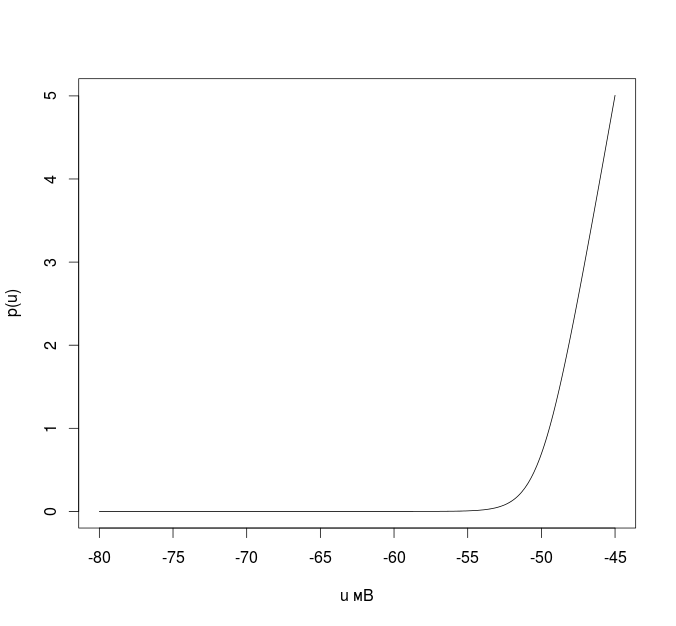
\includegraphics[width=1\linewidth]{p_srm}
\caption{Плотность вероятности генерации спайка}
\end{figure} \\
\indent Такая плотность вероятности является ненормализованной, т.к. её интеграл больше единицы, и имеет все свойства плотности вероятности Пуассоновского процесса. Например, вероятность генерации одного спайка в отрезок времени $\Delta t$ будет $P = p(u(t))\Delta t$. В данной работе взята функция вида
\begin{equation}\label{eq:p_dens}
p(u)=\frac{\beta}{\alpha}ln[1+exp(\alpha(U_{tresh}-v))]-\alpha(U_{tresh}-v)
\end{equation}
где константы $\alpha=\beta=1$, и порог $U_{tresh}$ по достижению которого функция резко растёт вверх равен -50 мВ.
\paragraph*{Математический фреймворк.} Используя выкладки выше можно вывести математическую базу для Spike Responce Model. Ниже приведены основные формулы.
\begin{itemize}
\item \textbf{Вероятность отсутствия спайков в диапазон $[0,T]$ при данных спайках на синапсах $X$ ($Y_{0} = \{\} $)}:
\begin{equation}\label{eq:p_y}
P(Y_{0}|X) = S[0,T] = \int_{0}^{T} exp(-p(t))dt\;,
\end{equation}
\\
\item \textbf{Вероятность генерации спайковой последовательности $Y = \{t_{f1},t_{f2},..,t_{fn}\}$ диапазоне $[0,T]$ при данных спайках на синапcах $X$.}
\begin{equation}\label{eq:p_y_complex}
P(Y|X)= S[0,t_{f1}]\; p(t_{f1})\;S[t_{f1},t_{f2}]\;p(t_{f2})...p(t_{fn}) \; S[t_{fn},T],
\end{equation}
что можно упростить, и считать только один интеграл:
\begin{equation}\label{eq:p_y}
P(Y|X)= S[0,T]\; p(t_{f1})\;p(t_{f2})\;...\;p(t_{fn})
\end{equation}
\end{itemize}
\paragraph*{Обучение.} При соединении таких SRM нейронов в сеть, имея набор входных спайков для каждого нейрона $X_{1}=\{t_{f1}^1, t_{f2}^1, ...,t_{fn}^1\}, X_{2}=\{t_{f1}^2, t_{f2}^2,...,t_{fn}^2\}$ и так далее, сеть будет порождать в определенной степени уникальный ответ в виде выходных спайков $Y=\{t_{f1}^Y, t_{f2}^Y,...,t_{fn}^Y\}$. Главный вопрос, который нужно поставить перед тем как обучать нашу модель - вопрос каким должен быть выходной ответ сети, и как он должен измениться во время обучения.\\
\indent Поставим задачу классификации и зададим требование, чтобы ответ сети для одного класса входных данных отличался от другого класса. Для выполнения этого требования необходимо, чтобы сеть выдавала наиболее постоянный, но, разумеется, не уникальный ответ, на все виды входных данных. Сеть построенная на SRM обладает не малой долей стохастичности и как одна из главных задач обучения таких сетей является задача снижения этой стохастичности, или иначе называя энтропии нейрона.\\
\indent Энтропию нейрона, как меру непредсказуемости его поведения, можно вывести используя классические уравнения из Теории Информации. Пусть $\xi$ - возможный ответ нейрона вида $[\sigma(0),\sigma(\Delta t),...,\sigma(T)]$, где $\sigma(t)=0$ если в данный момент нейрон не производил спайк и $\sigma(t)=1$, если спайк был. Множество всех возможных вариантов спайковых последовательностей обозначим через $\Omega$, причем $\xi\in\Omega$. Условная энтропия, при данном входе $X$, будет равна
\begin{equation}\label{eq:H}
H(\Omega|X) = -\;\int_{\Omega} p(\xi)log(\xi)d\xi
\end{equation}
где $p(\xi)$ - плотность вероятности спайковых последовательностей $\xi$.\\
\indent Снижая энтропию нейрона, нейрон обучается генерировать строго определенный набор выходных спайков для определенного входа, и в зависимости от разнородности входных спайковых последовательностей, нейрон будет генерировать разные выходные последовательности для разных классов. Перед тем как попытаться снизить энтропию нейрона, её необходимо измерить.\\
\indent Измерение энтропии всегда было трудоемкой задачей, так как влечет за собой измерение полной плотности вероятности. Математический фреймворк описанный выше позволяет вывести вероятность спайковой последовательности как функцию от входа $X$ и весов нейрона. Из-за рефракторности, нейрон, может производить ограниченный набор спайков в определенный момент времени и при сужении этого интервала, вероятность большого числа спайков становится меньше. Эту особенность можно использовать в контексте численного интегрирования \ref{eq:H} и посчитать интеграл только для ограниченного набора $\xi$:
\begin{itemize}
\item При отсутствии спайков на $[0,T]$
\begin{equation}\label{eq:H0}
H_{0}(\Omega_{0}|X) = -p_{0}\;log(p_{0}) 
\end{equation}
где $p_{0} = S[0,T]$, смотри \ref{eq:p_y}.
\item При наличии одного спайка на $[0,T]$
\begin{equation}\label{eq:H1}
H_{1}(\Omega_{1}|X) = -\int_{0}^{T} p_{1}(t_{f1})\;log(p_{1}(t_{f1})) dt_{f1}
\end{equation}
где $p_{1}(t_{f1}) = S[0,t_{f1}] \; p(t_{f1}) \; S[t_{f1},T]$
\item При наличии двух спайков на $[0,T]$
\begin{equation}\label{eq:H2}
H_{2}(\Omega_{2}|X) = -\int_{0}^{T} \int_{t_{f2}}^{T} p_{2}(t_{f1},t_{f2})\;log(p_{2}(t_{f1},t_{f2})) dt_{f1} dt_{f2}
\end{equation}
где $p_{2}(t_{f1},t_{f2}) = S[0,t_{f1}] \; p(t_{f1}) \;  S[t_{f1},t_{f2}] \;  p(t_{f2})\; S[t_{f2},T]$
\end{itemize}
\indent В итоге при выборе $T$, например, 20 мс, подсчет интеграла \label{eq:H} будет сводиться к сумме
\begin{equation}\label{eq:Hsum}
H(\Omega|X) = H_{0} + H_{1} + H_{2}
\end{equation}
причем энтропия нейрона при наличии трех спайков и более стремится к нулю, так как их вероятность предельно мала.
\paragraph*{Минимизация энтропии.} Функция вида \ref{eq:H} позволяет посчитать градиент изменения энтропии нейрона $i$ как функции весов
\begin{equation}\label{eq:Hgrad}
\frac{dH(\Omega|X)}{dw_{ij}} = -\int_{\Omega} p(\xi)\;(log(\xi)+1)\frac{dlog(p(\xi))}{dw_{ij}}d\xi
\end{equation}
причем
\begin{equation}\label{eq:dlog}
\frac{dlog(p(\xi))}{dw_{ij}} = -\int_{0}^{T} p'_{i}(t)\sum_{f_{j}\in \xi}\epsilon(t|f_{j})dt +\sum_{f_{i}\in Y}\frac{p'_{i}(f_{i})}{p_{i}(f_{i})}\epsilon(f_{i}|f_{j})
\end{equation}
где
\begin{equation}\label{eq:pstroke}
p'_{i}(t)=\frac{dp_{i}(t)}{du_{i}(t)} = \frac{\beta}{1+exp(\alpha(U_{tresh}-u_{i}(t))}
\end{equation}
\end{document}
